 \begin{appendices}

  \chapter{Class Documentation}
  
  \section{\-Hridd \-Class \-Reference}
\label{class_hridd}\index{\-Hridd@{\-Hridd}}
{\ttfamily \#include $<$\-Hridd.\-h$>$}

\begin{figure}[H]
\begin{center}
\leavevmode
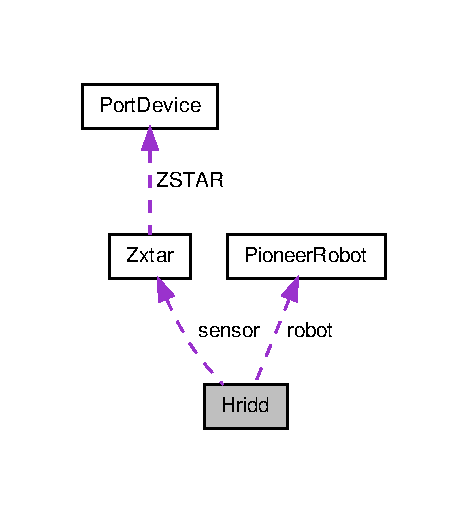
\includegraphics[width=225pt]{a}
\end{center}
\end{figure}

\subsubsection*{\-Public \-Member \-Functions}
\begin{itemize}
\item 
int {\bf \-Kbhit} (void)
\item 
void {\bf \-Gesture\-Control} ()
\item 
void {\bf \-Set\-A\-C\-C\-Frame\-Word} (unsigned int framevalue)
\end{itemize}

\subsubsection*{\-Public \-Attributes}
\begin{itemize}
\item 
{\bf \-Pioneer\-Robot} {\bf robot}
\item 
{\bf \-Zxtar} {\bf sensor}
\end{itemize}


\subsubsection{\-Detailed \-Description}
 \-Human-\/\-Robot \-Interaction \-Dance \-Demo class is aimed to combine the 
\-Zxtar class accelerometer class,  the Pioneer\-Robot class so as to control the robot with the user's wearable accelerometer.
\-Definition at line 16 of file \-Hridd.\-h.





\subsubsection{\-Member \-Function \-Documentation}
\index{\-Hridd@{\-Hridd}!\-Gesture\-Control@{\-Gesture\-Control}}
\index{\-Gesture\-Control@{\-Gesture\-Control}!Hridd@{\-Hridd}}
\paragraph[{\-Gesture\-Control}]{\setlength{\rightskip}{0pt plus 5cm}void {\bf \-Hridd\-::\-Gesture\-Control})}

\-This method contains the main control gesture for the robot movements 

\-Definition at line 40 of file \-Hridd.\-cpp.

\-Here is the call graph for this function\-:\nopagebreak
\begin{figure}[H]
\begin{center}
\leavevmode
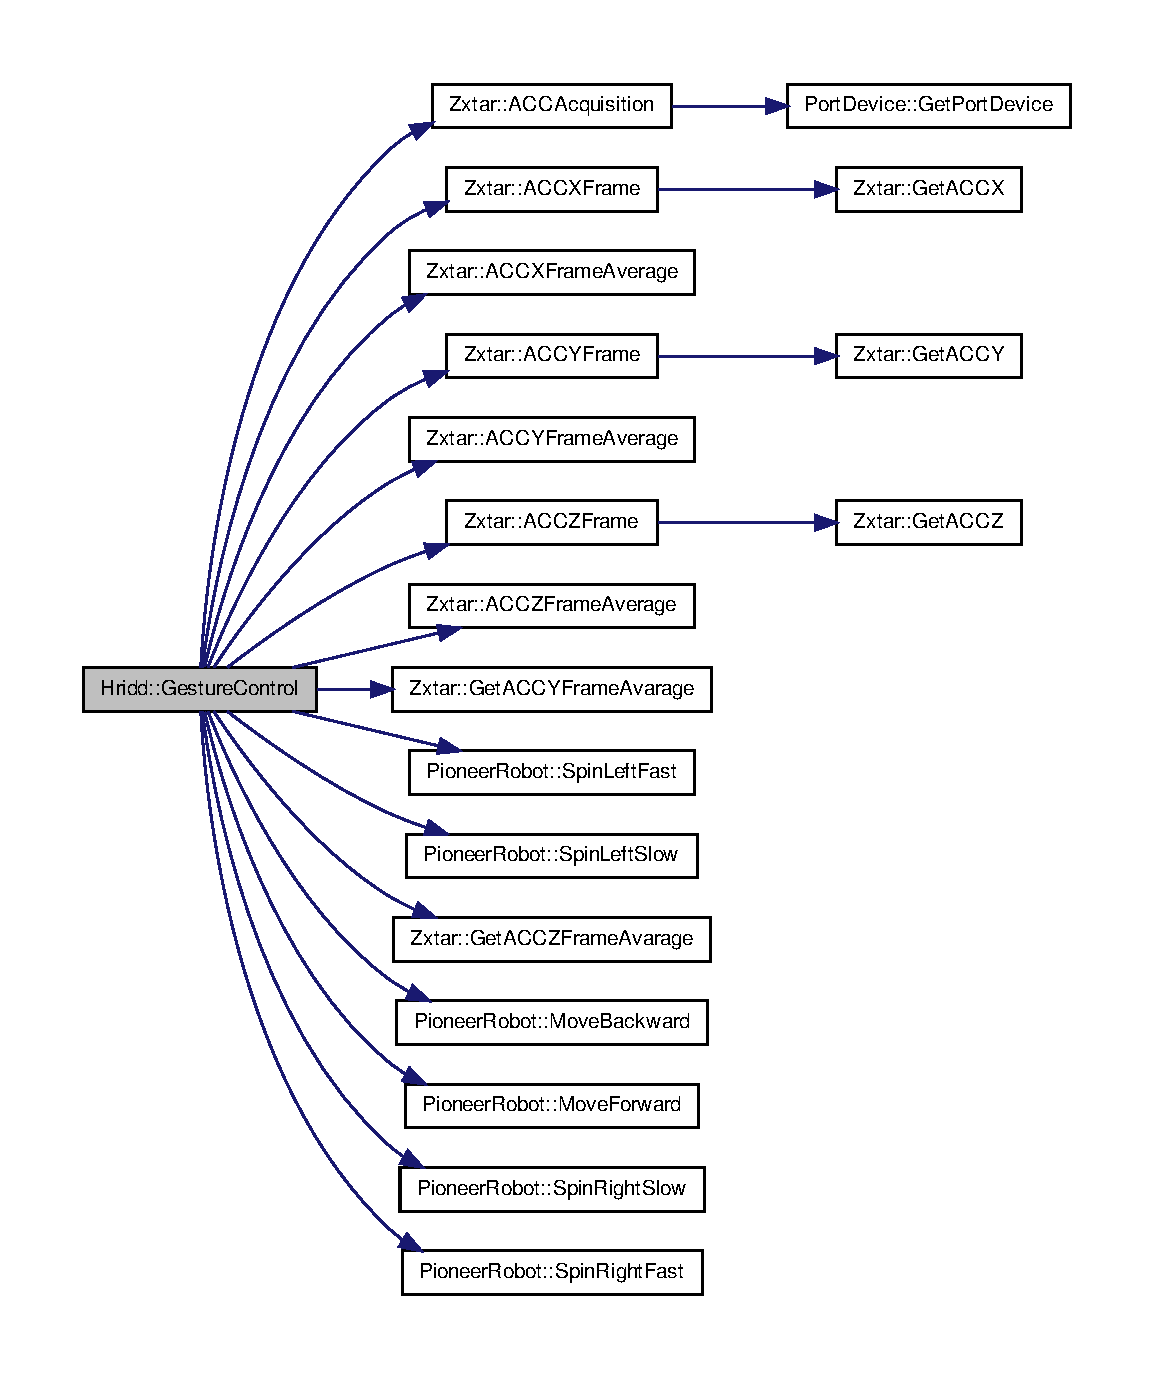
\includegraphics[width=350pt]{class_hridd_a0cb125f06d2dea3c85f2c88df2cf301b_cgraph}
\end{center}
\end{figure}





\index{\-Hridd@{\-Hridd}!\-Kbhit@{\-Kbhit}}
\index{\-Kbhit@{\-Kbhit}!Hridd@{\-Hridd}}
\paragraph[{\-Kbhit}]{\setlength{\rightskip}{0pt plus 5cm}int {\bf \-Hridd\-::\-Kbhit} (
)}\label{class_hridd_a4685da7617842bea560df152d2c5eb2e}
\-Method for the \-Keyboard hit 

\-Definition at line 8 of file \-Hridd.\-cpp.

\index{\-Hridd@{\-Hridd}!\-Set\-A\-C\-C\-Frame\-Word@{\-Set\-A\-C\-C\-Frame\-Word}}
\index{\-Set\-A\-C\-C\-Frame\-Word@{\-Set\-A\-C\-C\-Frame\-Word}!Hridd@{\-Hridd}}
\paragraph[{\-Set\-A\-C\-C\-Frame\-Word}]{\setlength{\rightskip}{0pt plus 5cm}void {\bf \-Hridd\-::\-Set\-A\-C\-C\-Frame\-Word} (
)}\label{class_hridd_ab782ddac948b4f7aca0596408cf5b714}
\-Function to set the \-Acceleration \-Frame \-Word 

\-Definition at line 34 of file \-Hridd.\-cpp.



\-Here is the call graph for this function\-:\nopagebreak
\begin{figure}[H]
\begin{center}
\leavevmode
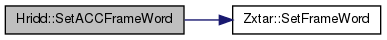
\includegraphics[width=350pt]{class_hridd_ab782ddac948b4f7aca0596408cf5b714_cgraph}
\end{center}
\end{figure}




\subsubsection{\-Member \-Data \-Documentation}
\index{\-Hridd@{\-Hridd}!robot@{robot}}
\index{robot@{robot}!Hridd@{\-Hridd}}
\paragraph[{robot}]{\setlength{\rightskip}{0pt plus 5cm}{\bf \-Pioneer\-Robot} {\bf \-Hridd\-::robot}}\label{class_hridd_a4d70b5a2dc5597c34e05023ffb84935d}
\-Data \-Member for the \-Pioner\-Robot \-Class which defines and initializes the robot 

\-Definition at line 23 of file \-Hridd.\-h.

\index{\-Hridd@{\-Hridd}!sensor@{sensor}}
\index{sensor@{sensor}!Hridd@{\-Hridd}}
\paragraph[{sensor}]{\setlength{\rightskip}{0pt plus 5cm}{\bf \-Zxtar} {\bf \-Hridd\-::sensor}}\label{class_hridd_a883c2d9756ee45e1c0be3b2ec359cee8}
\-Data \-Member for the \-Pioner\-Robot \-Class which defines and initializes the accelerometer sensor 

\-Definition at line 28 of file \-Hridd.\-h.




  \section{\-Pioneer\-Robot \-Class \-Reference}


\label{class_pioneer_robot}\index{\-Pioneer\-Robot@{\-Pioneer\-Robot}}


{\ttfamily \#include $<$\-Pioneer\-Robot.\-h$>$}

\subsubsection*{\-Public \-Member \-Functions}
\begin{itemize}
\item 
{\bf \-Pioneer\-Robot} ()
\item 
{\bf $\sim$\-Pioneer\-Robot} ()
\item 
virtual bool {\bf init} ()
\item 
virtual void {\bf get\-Current\-Configuration} (std\-::vector$<$ double $>$ \&q)
\item 
virtual bool {\bf move\-To\-Configuration} (std\-::vector$<$ double $>$ configuration)
\item 
void {\bf \-Move\-Forward} ()
\item 
void {\bf \-Move\-Backward} ()
\item 
void {\bf \-Spin\-Left\-Slow} ()
\item 
void {\bf \-Spin\-Right\-Slow} ()
\item 
void {\bf \-Spin\-Left\-Fast} ()
\item 
void {\bf \-Spin\-Right\-Fast} ()
\end{itemize}
\subsubsection*{\-Public \-Attributes}
\begin{itemize}
\item 
\-Ar\-Robot {\bf pioneer}
\end{itemize}
\subsubsection*{\-Protected \-Member \-Functions}
\begin{itemize}
\item 
double {\bf validate\-Angle} (double angle)
\end{itemize}


\subsubsection{\-Detailed \-Description}


\-Definition at line 13 of file \-Pioneer\-Robot.\-h.



\subsubsection{\-Constructor \& \-Destructor \-Documentation}
\index{\-Pioneer\-Robot@{\-Pioneer\-Robot}!\-Pioneer\-Robot@{\-Pioneer\-Robot}}
\index{\-Pioneer\-Robot@{\-Pioneer\-Robot}!PioneerRobot@{\-Pioneer\-Robot}}
\paragraph[{\-Pioneer\-Robot}]{\setlength{\rightskip}{0pt plus 5cm}{\bf \-Pioneer\-Robot\-::\-Pioneer\-Robot} (
)}\label{class_pioneer_robot_aa90f53954d9e38db6e7ece95439fafae}


\-Definition at line 3 of file \-Pioneer\-Robot.\-cpp.



\-Here is the call graph for this function\-:\nopagebreak
\begin{figure}[H]
\begin{center}
\leavevmode
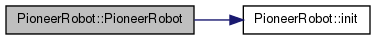
\includegraphics[width=350pt]{class_pioneer_robot_aa90f53954d9e38db6e7ece95439fafae_cgraph}
\end{center}
\end{figure}


\index{\-Pioneer\-Robot@{\-Pioneer\-Robot}!$\sim$\-Pioneer\-Robot@{$\sim$\-Pioneer\-Robot}}
\index{$\sim$\-Pioneer\-Robot@{$\sim$\-Pioneer\-Robot}!PioneerRobot@{\-Pioneer\-Robot}}
\paragraph[{$\sim$\-Pioneer\-Robot}]{\setlength{\rightskip}{0pt plus 5cm}{\bf \-Pioneer\-Robot\-::$\sim$\-Pioneer\-Robot} (
)}\label{class_pioneer_robot_af543718d0dc3bceef69c9fb2f604b701}


\-Definition at line 9 of file \-Pioneer\-Robot.\-cpp.



\subsubsection{\-Member \-Function \-Documentation}
\index{\-Pioneer\-Robot@{\-Pioneer\-Robot}!get\-Current\-Configuration@{get\-Current\-Configuration}}
\index{get\-Current\-Configuration@{get\-Current\-Configuration}!PioneerRobot@{\-Pioneer\-Robot}}
\paragraph[{get\-Current\-Configuration}]{\setlength{\rightskip}{0pt plus 5cm}void {\bf \-Pioneer\-Robot\-::get\-Current\-Configuration} (
\begin{itemize}
\item[{std\-::vector$<$ double $>$ \&}]{q}
\end{itemize}
)\hspace{0.3cm}{\ttfamily  [virtual]}}\label{class_pioneer_robot_a42cb581f7beeb71717951d9ae78e035b}


\-Definition at line 76 of file \-Pioneer\-Robot.\-cpp.

\index{\-Pioneer\-Robot@{\-Pioneer\-Robot}!init@{init}}
\index{init@{init}!PioneerRobot@{\-Pioneer\-Robot}}
\paragraph[{init}]{\setlength{\rightskip}{0pt plus 5cm}bool {\bf \-Pioneer\-Robot\-::init} (
)\hspace{0.3cm}{\ttfamily  [virtual]}}\label{class_pioneer_robot_a1524060d928fa3bb448c8cc7ef08f3cf}


\-Definition at line 15 of file \-Pioneer\-Robot.\-cpp.

\index{\-Pioneer\-Robot@{\-Pioneer\-Robot}!\-Move\-Backward@{\-Move\-Backward}}
\index{\-Move\-Backward@{\-Move\-Backward}!PioneerRobot@{\-Pioneer\-Robot}}
\paragraph[{\-Move\-Backward}]{\setlength{\rightskip}{0pt plus 5cm}void {\bf \-Pioneer\-Robot\-::\-Move\-Backward} (
)}\label{class_pioneer_robot_aadf2a82ec535334ac57d216d98abc023}


\-Definition at line 144 of file \-Pioneer\-Robot.\-cpp.

\index{\-Pioneer\-Robot@{\-Pioneer\-Robot}!\-Move\-Forward@{\-Move\-Forward}}
\index{\-Move\-Forward@{\-Move\-Forward}!PioneerRobot@{\-Pioneer\-Robot}}
\paragraph[{\-Move\-Forward}]{\setlength{\rightskip}{0pt plus 5cm}void {\bf \-Pioneer\-Robot\-::\-Move\-Forward} (
)}\label{class_pioneer_robot_a017c9e7b9a409f07f71f152024e927b9}


\-Definition at line 149 of file \-Pioneer\-Robot.\-cpp.

\index{\-Pioneer\-Robot@{\-Pioneer\-Robot}!move\-To\-Configuration@{move\-To\-Configuration}}
\index{move\-To\-Configuration@{move\-To\-Configuration}!PioneerRobot@{\-Pioneer\-Robot}}
\paragraph[{move\-To\-Configuration}]{\setlength{\rightskip}{0pt plus 5cm}bool {\bf \-Pioneer\-Robot\-::move\-To\-Configuration} (
\begin{itemize}
\item[{std\-::vector$<$ double $>$}]{configuration}
\end{itemize}
)\hspace{0.3cm}{\ttfamily  [virtual]}}\label{class_pioneer_robot_a911225fb4f2611d77f5e2c9185098bec}


\-Definition at line 91 of file \-Pioneer\-Robot.\-cpp.

\index{\-Pioneer\-Robot@{\-Pioneer\-Robot}!\-Spin\-Left\-Fast@{\-Spin\-Left\-Fast}}
\index{\-Spin\-Left\-Fast@{\-Spin\-Left\-Fast}!PioneerRobot@{\-Pioneer\-Robot}}
\paragraph[{\-Spin\-Left\-Fast}]{\setlength{\rightskip}{0pt plus 5cm}void {\bf \-Pioneer\-Robot\-::\-Spin\-Left\-Fast} (
)}\label{class_pioneer_robot_a4d151faa33be37f7ce1da5d59c907dc1}


\-Definition at line 164 of file \-Pioneer\-Robot.\-cpp.

\index{\-Pioneer\-Robot@{\-Pioneer\-Robot}!\-Spin\-Left\-Slow@{\-Spin\-Left\-Slow}}
\index{\-Spin\-Left\-Slow@{\-Spin\-Left\-Slow}!PioneerRobot@{\-Pioneer\-Robot}}
\paragraph[{\-Spin\-Left\-Slow}]{\setlength{\rightskip}{0pt plus 5cm}void {\bf \-Pioneer\-Robot\-::\-Spin\-Left\-Slow} (
)}\label{class_pioneer_robot_a604a97dddb6910bb7ea086fd521c01fd}


\-Definition at line 154 of file \-Pioneer\-Robot.\-cpp.

\index{\-Pioneer\-Robot@{\-Pioneer\-Robot}!\-Spin\-Right\-Fast@{\-Spin\-Right\-Fast}}
\index{\-Spin\-Right\-Fast@{\-Spin\-Right\-Fast}!PioneerRobot@{\-Pioneer\-Robot}}
\paragraph[{\-Spin\-Right\-Fast}]{\setlength{\rightskip}{0pt plus 5cm}void {\bf \-Pioneer\-Robot\-::\-Spin\-Right\-Fast} (
)}\label{class_pioneer_robot_afe663e18d34e3dc9bf3988df958f691d}


\-Definition at line 169 of file \-Pioneer\-Robot.\-cpp.

\index{\-Pioneer\-Robot@{\-Pioneer\-Robot}!\-Spin\-Right\-Slow@{\-Spin\-Right\-Slow}}
\index{\-Spin\-Right\-Slow@{\-Spin\-Right\-Slow}!PioneerRobot@{\-Pioneer\-Robot}}
\paragraph[{\-Spin\-Right\-Slow}]{\setlength{\rightskip}{0pt plus 5cm}void {\bf \-Pioneer\-Robot\-::\-Spin\-Right\-Slow} (
)}\label{class_pioneer_robot_a976e2d9dcc5396b52ea323cce8d4f45a}


\-Definition at line 159 of file \-Pioneer\-Robot.\-cpp.

\index{\-Pioneer\-Robot@{\-Pioneer\-Robot}!validate\-Angle@{validate\-Angle}}
\index{validate\-Angle@{validate\-Angle}!PioneerRobot@{\-Pioneer\-Robot}}
\paragraph[{validate\-Angle}]{\setlength{\rightskip}{0pt plus 5cm}double {\bf \-Pioneer\-Robot\-::validate\-Angle} (
\begin{itemize}
\item[{double}]{angle}
\end{itemize}
)\hspace{0.3cm}{\ttfamily  [protected]}}\label{class_pioneer_robot_a418d07d081a9451edd4b7d7af804e926}


\-Definition at line 132 of file \-Pioneer\-Robot.\-cpp.



\subsubsection{\-Member \-Data \-Documentation}
\index{\-Pioneer\-Robot@{\-Pioneer\-Robot}!pioneer@{pioneer}}
\index{pioneer@{pioneer}!PioneerRobot@{\-Pioneer\-Robot}}
\paragraph[{pioneer}]{\setlength{\rightskip}{0pt plus 5cm}\-Ar\-Robot {\bf \-Pioneer\-Robot\-::pioneer}}\label{class_pioneer_robot_a05e2fbb4d51eef3358e122508cdbfbfb}


\-Definition at line 31 of file \-Pioneer\-Robot.\-h.


  
  
  
  
    \section{\-Port\-Device \-Class \-Reference}
\label{class_port_device}\index{\-Port\-Device@{\-Port\-Device}}


{\ttfamily \#include $<$\-Port\-Device.\-h$>$}

\subsubsection*{\-Public \-Member \-Functions}
\begin{itemize}
\item 
{\bf \-Port\-Device} ()
\item 
int {\bf \-Allocate\-Port\-Device} ()
\item 
int {\bf \-Config\-Port\-Device} ()
\item 
int {\bf \-Get\-Port\-Device} ()
\item 
void {\bf \-Clean\-Port\-Device} ()
\item 
void {\bf \-Close\-Port\-Device} ()
\end{itemize}


\subsubsection{\-Detailed \-Description}


\-Definition at line 27 of file \-Port\-Device.\-h.



\subsubsection{\-Constructor \& \-Destructor \-Documentation}
\index{\-Port\-Device@{\-Port\-Device}!\-Port\-Device@{\-Port\-Device}}
\index{\-Port\-Device@{\-Port\-Device}!PortDevice@{\-Port\-Device}}
\paragraph[{\-Port\-Device}]{\setlength{\rightskip}{0pt plus 5cm}{\bf \-Port\-Device\-::\-Port\-Device} (
)}\label{class_port_device_a12ea5f06d1850a4ef58b89f2c94c2039}
\-Constructor to reset, to allocate and configurate the \-Z\-S\-T\-A\-R \-U\-S\-B \-Stick 

\-Definition at line 4 of file \-Port\-Device.\-cpp.



\-Here is the call graph for this function\-:\nopagebreak
\begin{figure}[H]
\begin{center}
\leavevmode
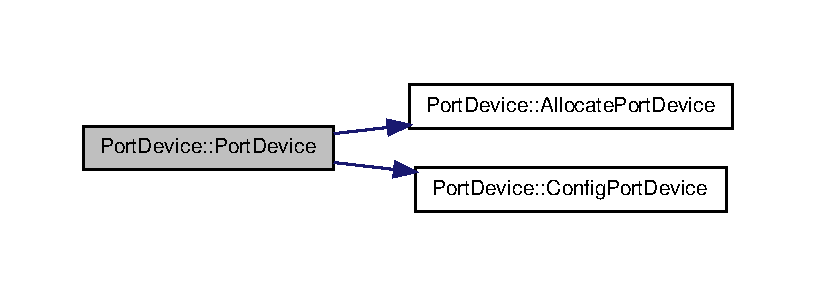
\includegraphics[width=350pt]{class_port_device_a12ea5f06d1850a4ef58b89f2c94c2039_cgraph}
\end{center}
\end{figure}




\subsubsection{\-Member \-Function \-Documentation}
\index{\-Port\-Device@{\-Port\-Device}!\-Allocate\-Port\-Device@{\-Allocate\-Port\-Device}}
\index{\-Allocate\-Port\-Device@{\-Allocate\-Port\-Device}!PortDevice@{\-Port\-Device}}
\paragraph[{\-Allocate\-Port\-Device}]{\setlength{\rightskip}{0pt plus 5cm}int {\bf \-Port\-Device\-::\-Allocate\-Port\-Device} (
)}\label{class_port_device_ac93ffc96c1a14ee5d4b9eed9fb17d103}
\-Set\-Port\-Device\-F\-D 

\-Definition at line 13 of file \-Port\-Device.\-cpp.

\index{\-Port\-Device@{\-Port\-Device}!\-Clean\-Port\-Device@{\-Clean\-Port\-Device}}
\index{\-Clean\-Port\-Device@{\-Clean\-Port\-Device}!PortDevice@{\-Port\-Device}}
\paragraph[{\-Clean\-Port\-Device}]{\setlength{\rightskip}{0pt plus 5cm}void {\bf \-Port\-Device\-::\-Clean\-Port\-Device} (
)}\label{class_port_device_ab961a8d36a509d74ec73560ecf8e08c3}
function to clean the \-Port \-Device 

\-Definition at line 89 of file \-Port\-Device.\-cpp.

\index{\-Port\-Device@{\-Port\-Device}!\-Close\-Port\-Device@{\-Close\-Port\-Device}}
\index{\-Close\-Port\-Device@{\-Close\-Port\-Device}!PortDevice@{\-Port\-Device}}
\paragraph[{\-Close\-Port\-Device}]{\setlength{\rightskip}{0pt plus 5cm}void {\bf \-Port\-Device\-::\-Close\-Port\-Device} (
)}\label{class_port_device_a46070f7913dc823c394a5420efbe1e20}
\-Close\-Port\-Device 

\-Definition at line 83 of file \-Port\-Device.\-cpp.

\index{\-Port\-Device@{\-Port\-Device}!\-Config\-Port\-Device@{\-Config\-Port\-Device}}
\index{\-Config\-Port\-Device@{\-Config\-Port\-Device}!PortDevice@{\-Port\-Device}}
\paragraph[{\-Config\-Port\-Device}]{\setlength{\rightskip}{0pt plus 5cm}int {\bf \-Port\-Device\-::\-Config\-Port\-Device} (
)}\label{class_port_device_a40bbaa8614cadd8420fa32a72024aa0a}
\-Config\-Port\-Device\-F\-D 

\-Definition at line 28 of file \-Port\-Device.\-cpp.

\index{\-Port\-Device@{\-Port\-Device}!\-Get\-Port\-Device@{\-Get\-Port\-Device}}
\index{\-Get\-Port\-Device@{\-Get\-Port\-Device}!PortDevice@{\-Port\-Device}}
\paragraph[{\-Get\-Port\-Device}]{\setlength{\rightskip}{0pt plus 5cm}int {\bf \-Port\-Device\-::\-Get\-Port\-Device} (
)}\label{class_port_device_a385e13c178d6d8b61688e7df29e43f71}
function to get the port's \-F\-I\-L\-E \-D\-E\-S\-C\-R\-I\-P\-T\-O\-R 

\-Definition at line 78 of file \-Port\-Device.\-cpp.


  
  
  
  
    \section{\-Zxtar \-Class \-Reference}
\label{class_zxtar}\index{\-Zxtar@{\-Zxtar}}


{\ttfamily \#include $<$\-Zxtar.\-h$>$}



\-Collaboration diagram for \-Zxtar\-:\nopagebreak
\begin{figure}[H]
\begin{center}
\leavevmode
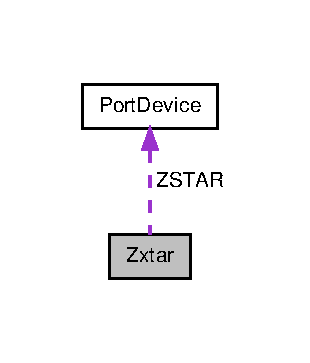
\includegraphics[width=149pt]{class_zxtar__coll__graph}
\end{center}
\end{figure}
\subsubsection*{\-Public \-Member \-Functions}
\begin{itemize}
\item 
{\bf \-Zxtar} ()
\item 
{\bf \-Zxtar} (int g\-Sensitivity, int set\-Rate)
\item 
void {\bf \-Available\-A\-C\-C} ()
\item 
int {\bf \-Kbhit} (void)
\item 
void {\bf \-Set\-Sensitivity} (int g\-Sensitivity)
\item 
void {\bf \-Data\-Rate} (int set\-Rate)
\item 
void {\bf \-A\-C\-C\-Acquisition} ()
\item 
double {\bf \-Get\-A\-C\-C\-X} ()
\item 
double {\bf \-Get\-A\-C\-C\-Y} ()
\item 
double {\bf \-Get\-A\-C\-C\-Z} ()
\item 
void {\bf \-A\-C\-C\-Print} ()
\item 
void {\bf start\-Timer} ()
\item 
double {\bf stop\-Timer} ()
\item 
void {\bf \-Set\-Frame\-Word} (unsigned int framevalue)
\item 
void {\bf \-A\-C\-C\-X\-Frame} ()
\item 
void {\bf \-A\-C\-C\-X\-Frame\-Print} ()
\item 
double {\bf \-A\-C\-C\-X\-Frame\-Average} ()
\item 
double {\bf \-Get\-A\-C\-C\-X\-Frame\-Avarage} ()
\item 
double {\bf \-A\-C\-C\-X\-Frame\-Std\-Deviation} ()
\item 
double {\bf \-Get\-A\-C\-C\-X\-Frame\-Std\-Deviation} ()
\item 
void {\bf \-A\-C\-C\-Y\-Frame} ()
\item 
void {\bf \-A\-C\-C\-Y\-Frame\-Print} ()
\item 
double {\bf \-A\-C\-C\-Y\-Frame\-Average} ()
\item 
double {\bf \-Get\-A\-C\-C\-Y\-Frame\-Avarage} ()
\item 
double {\bf \-A\-C\-C\-Y\-Frame\-Std\-Deviation} ()
\item 
double {\bf \-Get\-A\-C\-C\-Y\-Frame\-Std\-Deviation} ()
\item 
void {\bf \-A\-C\-C\-Z\-Frame} ()
\item 
void {\bf \-A\-C\-C\-Z\-Frame\-Print} ()
\item 
double {\bf \-A\-C\-C\-Z\-Frame\-Average} ()
\item 
double {\bf \-Get\-A\-C\-C\-Z\-Frame\-Avarage} ()
\item 
double {\bf \-A\-C\-C\-Z\-Frame\-Std\-Deviation} ()
\item 
double {\bf \-Get\-A\-C\-C\-Z\-Frame\-Std\-Deviation} ()
\end{itemize}
\subsubsection*{\-Static \-Public \-Member \-Functions}
\begin{itemize}
\item 
static void {\bf print\-Time} (double duration)
\end{itemize}
\subsubsection*{\-Public \-Attributes}
\begin{itemize}
\item 
{\bf \-Port\-Device} {\bf \-Z\-S\-T\-A\-R}
\end{itemize}


\subsubsection{\-Detailed \-Description}
\-Zxtar class permitis to extract a frame, and compute the avarage and \-Standar \-Deviation, as well to get these values for the \-X, \-Y and \-Z axis. \-The following code is an example for its use; uncomment the code for further test.

\-Zxtar sensor; // \-Declaration of the sensor \-Zstar class type

sensor.\-A\-C\-C\-X\-Frame(); // \-Getting the \-A\-C\-C of the \-X-\/axis frame word

sensor.\-A\-C\-C\-X\-Frame\-Average(); // \-X-\/axis \-A\-C\-C frame mean

sensor.\-A\-C\-C\-X\-Frame\-Std\-Deviation(); // \-X-\/axis \-A\-C\-C frame \-Standard \-Deviation

cout $<$$<$ sensor.\-Get\-A\-C\-C\-X\-Frame\-Avarage() $<$$<$ endl; //\-Printing the \-A\-C\-C\-X value of the frame avarage

cout $<$$<$ sensor.\-Get\-A\-C\-C\-X\-Frame\-Std\-Deviation() $<$$<$ endl; //\-Printing the \-A\-C\-C\-X value of the frame standard deviation 

\-Definition at line 47 of file \-Zxtar.\-h.



\subsubsection{\-Constructor \& \-Destructor \-Documentation}
\index{\-Zxtar@{\-Zxtar}!\-Zxtar@{\-Zxtar}}
\index{\-Zxtar@{\-Zxtar}!Zxtar@{\-Zxtar}}
\paragraph[{\-Zxtar}]{\setlength{\rightskip}{0pt plus 5cm}{\bf \-Zxtar\-::\-Zxtar} (
)}\label{class_zxtar_ade1535d0a5d35149f616eabc03838bba}
\-Default \-Constructor with the default values for sensitibility and data rate\-: 2g and 60\-Hz 

\-Definition at line 4 of file \-Zxtar.\-cpp.



\-Here is the call graph for this function\-:\nopagebreak
\begin{figure}[H]
\begin{center}
\leavevmode
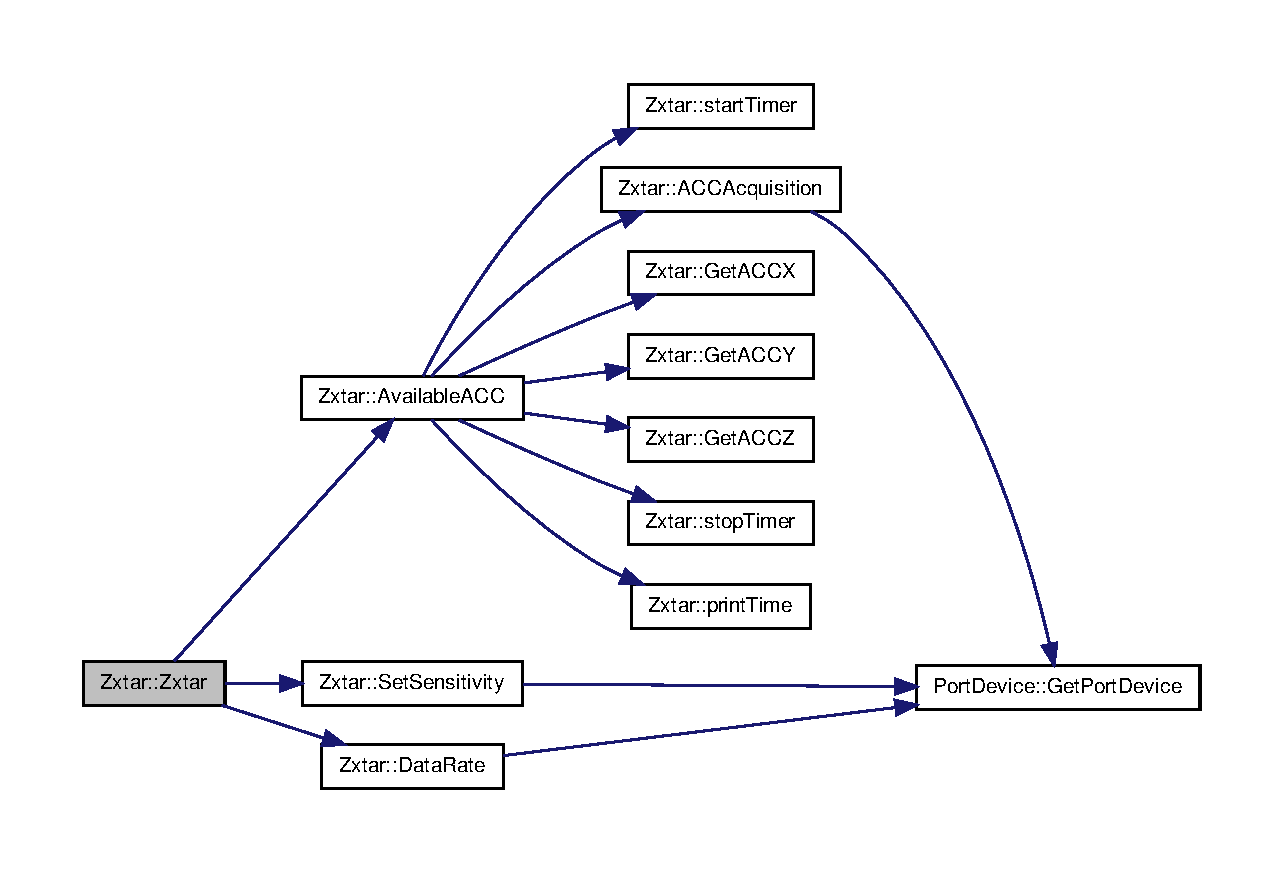
\includegraphics[width=350pt]{class_zxtar_ade1535d0a5d35149f616eabc03838bba_cgraph}
\end{center}
\end{figure}


\index{\-Zxtar@{\-Zxtar}!\-Zxtar@{\-Zxtar}}
\index{\-Zxtar@{\-Zxtar}!Zxtar@{\-Zxtar}}
\paragraph[{\-Zxtar}]{\setlength{\rightskip}{0pt plus 5cm}{\bf \-Zxtar\-::\-Zxtar} (
\begin{itemize}
\item[{int}]{g\-Sensitivity, }
\item[{int}]{set\-Rate}
\end{itemize}
)}\label{class_zxtar_ad47b8fe7f2075b0c8e15925adbe46551}
\-Constructor with parameter options, so as the user is able to configure the sensor by using the following values

\-Zxtar name(g-\/range, \-Data\-Rate);

..............$|$........$|$

.............$|$........$|$-\/-\/-\/-\/-\/-\/-\/-\/-\/ \-Available \-Values for \-Data\-Rate are 30, 60, and 120

.............$|$-\/-\/-\/-\/-\/-\/-\/-\/-\/-\/-\/-\/-\/-\/-\/-\/-\/-\/-\/ \-Available \-Values for g-\/range parameter are 2, 4, and 8. 

\-Definition at line 21 of file \-Zxtar.\-cpp.



\-Here is the call graph for this function\-:\nopagebreak
\begin{figure}[H]
\begin{center}
\leavevmode
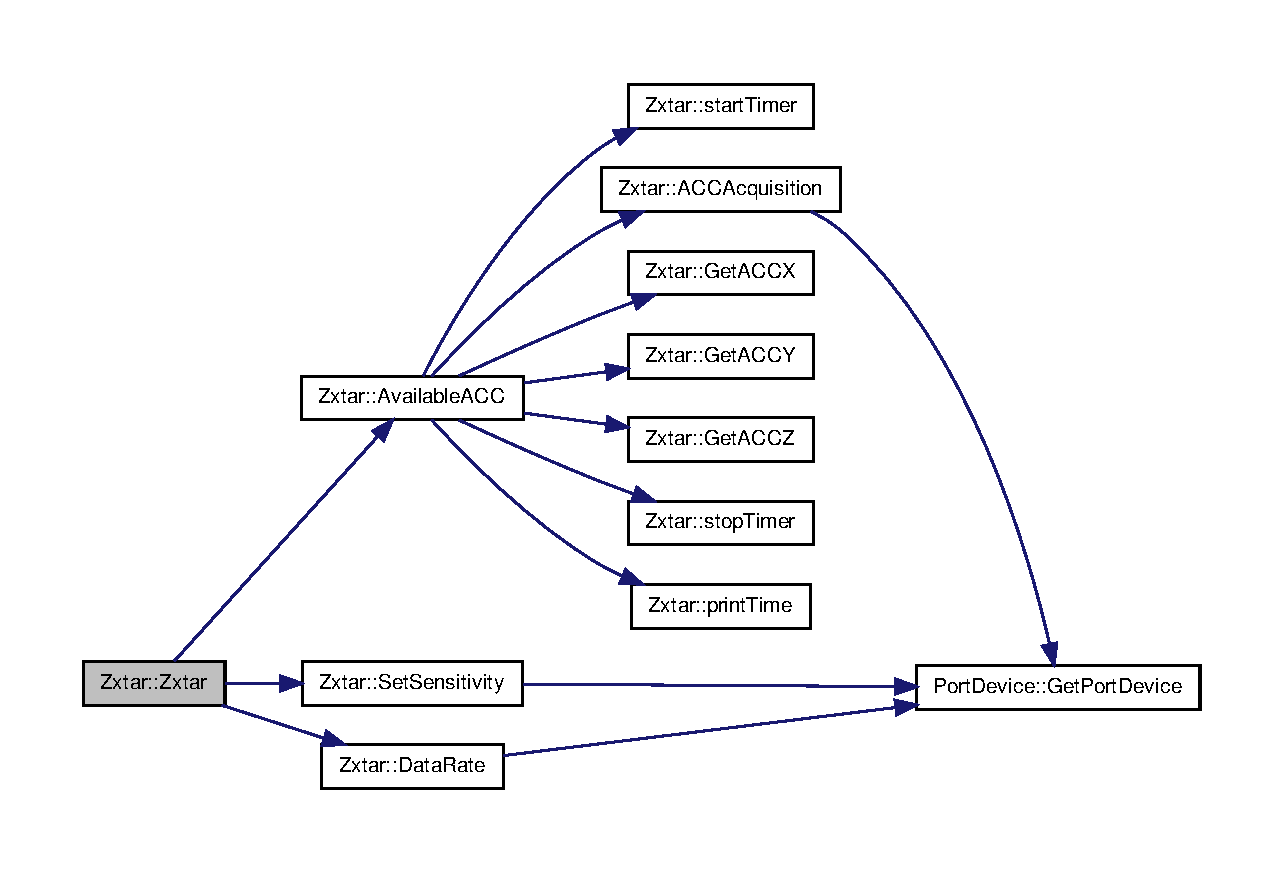
\includegraphics[width=350pt]{class_zxtar_ad47b8fe7f2075b0c8e15925adbe46551_cgraph}
\end{center}
\end{figure}




\subsubsection{\-Member \-Function \-Documentation}
\index{\-Zxtar@{\-Zxtar}!\-A\-C\-C\-Acquisition@{\-A\-C\-C\-Acquisition}}
\index{\-A\-C\-C\-Acquisition@{\-A\-C\-C\-Acquisition}!Zxtar@{\-Zxtar}}
\paragraph[{\-A\-C\-C\-Acquisition}]{\setlength{\rightskip}{0pt plus 5cm}void {\bf \-Zxtar\-::\-A\-C\-C\-Acquisition} (
)}\label{class_zxtar_ac5fb3cd141135976bd9edd5d05b7e95e}
\-Method for the \-Acceleration \-Acquisition 

\-Definition at line 149 of file \-Zxtar.\-cpp.



\-Here is the call graph for this function\-:\nopagebreak
\begin{figure}[H]
\begin{center}
\leavevmode
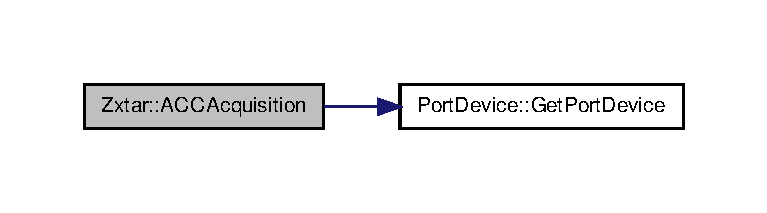
\includegraphics[width=350pt]{class_zxtar_ac5fb3cd141135976bd9edd5d05b7e95e_cgraph}
\end{center}
\end{figure}


\index{\-Zxtar@{\-Zxtar}!\-A\-C\-C\-Print@{\-A\-C\-C\-Print}}
\index{\-A\-C\-C\-Print@{\-A\-C\-C\-Print}!Zxtar@{\-Zxtar}}
\paragraph[{\-A\-C\-C\-Print}]{\setlength{\rightskip}{0pt plus 5cm}void {\bf \-Zxtar\-::\-A\-C\-C\-Print} (
)}\label{class_zxtar_a44686177358c40f3646c6e88d997296c}
\-Method to print the \-Acceleartion \-Values 

\-Definition at line 186 of file \-Zxtar.\-cpp.



\-Here is the call graph for this function\-:\nopagebreak
\begin{figure}[H]
\begin{center}
\leavevmode
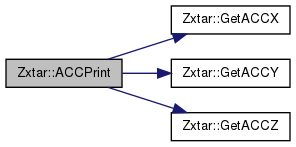
\includegraphics[width=294pt]{class_zxtar_a44686177358c40f3646c6e88d997296c_cgraph}
\end{center}
\end{figure}


\index{\-Zxtar@{\-Zxtar}!\-A\-C\-C\-X\-Frame@{\-A\-C\-C\-X\-Frame}}
\index{\-A\-C\-C\-X\-Frame@{\-A\-C\-C\-X\-Frame}!Zxtar@{\-Zxtar}}
\paragraph[{\-A\-C\-C\-X\-Frame}]{\setlength{\rightskip}{0pt plus 5cm}void {\bf \-Zxtar\-::\-A\-C\-C\-X\-Frame} (
)}\label{class_zxtar_aaef8fc83168462e070d4eb2884c6faba}
\-Method for the adquisition of \-X-\/axis data frame 

\-Definition at line 234 of file \-Zxtar.\-cpp.



\-Here is the call graph for this function\-:\nopagebreak
\begin{figure}[H]
\begin{center}
\leavevmode
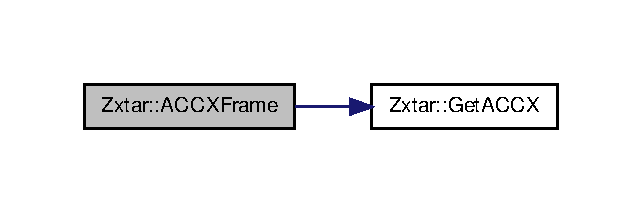
\includegraphics[width=308pt]{class_zxtar_aaef8fc83168462e070d4eb2884c6faba_cgraph}
\end{center}
\end{figure}


\index{\-Zxtar@{\-Zxtar}!\-A\-C\-C\-X\-Frame\-Average@{\-A\-C\-C\-X\-Frame\-Average}}
\index{\-A\-C\-C\-X\-Frame\-Average@{\-A\-C\-C\-X\-Frame\-Average}!Zxtar@{\-Zxtar}}
\paragraph[{\-A\-C\-C\-X\-Frame\-Average}]{\setlength{\rightskip}{0pt plus 5cm}double {\bf \-Zxtar\-::\-A\-C\-C\-X\-Frame\-Average} (
)}\label{class_zxtar_a8623ff9e740e0d6068f8b85ba2499a24}
\-Method to compute the \-X-\/axis data frame avarage 

\-Definition at line 261 of file \-Zxtar.\-cpp.

\index{\-Zxtar@{\-Zxtar}!\-A\-C\-C\-X\-Frame\-Print@{\-A\-C\-C\-X\-Frame\-Print}}
\index{\-A\-C\-C\-X\-Frame\-Print@{\-A\-C\-C\-X\-Frame\-Print}!Zxtar@{\-Zxtar}}
\paragraph[{\-A\-C\-C\-X\-Frame\-Print}]{\setlength{\rightskip}{0pt plus 5cm}void {\bf \-Zxtar\-::\-A\-C\-C\-X\-Frame\-Print} (
)}\label{class_zxtar_ac91d12d80e2b50ca915f83395890a420}
\-Method for printing the \-X-\/axis data frame 

\-Definition at line 248 of file \-Zxtar.\-cpp.

\index{\-Zxtar@{\-Zxtar}!\-A\-C\-C\-X\-Frame\-Std\-Deviation@{\-A\-C\-C\-X\-Frame\-Std\-Deviation}}
\index{\-A\-C\-C\-X\-Frame\-Std\-Deviation@{\-A\-C\-C\-X\-Frame\-Std\-Deviation}!Zxtar@{\-Zxtar}}
\paragraph[{\-A\-C\-C\-X\-Frame\-Std\-Deviation}]{\setlength{\rightskip}{0pt plus 5cm}double {\bf \-Zxtar\-::\-A\-C\-C\-X\-Frame\-Std\-Deviation} (
)}\label{class_zxtar_abc19d82ccb30e8cb23e017fb0c9f028b}
\-Method to compute the \-X-\/axis data frame standard deviation 

\-Definition at line 282 of file \-Zxtar.\-cpp.

\index{\-Zxtar@{\-Zxtar}!\-A\-C\-C\-Y\-Frame@{\-A\-C\-C\-Y\-Frame}}
\index{\-A\-C\-C\-Y\-Frame@{\-A\-C\-C\-Y\-Frame}!Zxtar@{\-Zxtar}}
\paragraph[{\-A\-C\-C\-Y\-Frame}]{\setlength{\rightskip}{0pt plus 5cm}void {\bf \-Zxtar\-::\-A\-C\-C\-Y\-Frame} (
)}\label{class_zxtar_a199057b6f8e74055b3c275ee2b2b1ea1}
\-Method for the adquisition of \-Y-\/axis data frame 

\-Definition at line 304 of file \-Zxtar.\-cpp.



\-Here is the call graph for this function\-:\nopagebreak
\begin{figure}[H]
\begin{center}
\leavevmode
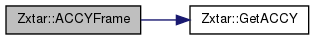
\includegraphics[width=308pt]{class_zxtar_a199057b6f8e74055b3c275ee2b2b1ea1_cgraph}
\end{center}
\end{figure}


\index{\-Zxtar@{\-Zxtar}!\-A\-C\-C\-Y\-Frame\-Average@{\-A\-C\-C\-Y\-Frame\-Average}}
\index{\-A\-C\-C\-Y\-Frame\-Average@{\-A\-C\-C\-Y\-Frame\-Average}!Zxtar@{\-Zxtar}}
\paragraph[{\-A\-C\-C\-Y\-Frame\-Average}]{\setlength{\rightskip}{0pt plus 5cm}double {\bf \-Zxtar\-::\-A\-C\-C\-Y\-Frame\-Average} (
)}\label{class_zxtar_a2ae4a211920a7ed0709956aa2d378508}
\-Method to compute the \-Y-\/axis data frame avarage 

\-Definition at line 331 of file \-Zxtar.\-cpp.

\index{\-Zxtar@{\-Zxtar}!\-A\-C\-C\-Y\-Frame\-Print@{\-A\-C\-C\-Y\-Frame\-Print}}
\index{\-A\-C\-C\-Y\-Frame\-Print@{\-A\-C\-C\-Y\-Frame\-Print}!Zxtar@{\-Zxtar}}
\paragraph[{\-A\-C\-C\-Y\-Frame\-Print}]{\setlength{\rightskip}{0pt plus 5cm}void {\bf \-Zxtar\-::\-A\-C\-C\-Y\-Frame\-Print} (
)}\label{class_zxtar_aa65c533b4afabe807a8c603a3538c3a3}
\-Method for printing the \-Y-\/axis data frame 

\-Definition at line 318 of file \-Zxtar.\-cpp.

\index{\-Zxtar@{\-Zxtar}!\-A\-C\-C\-Y\-Frame\-Std\-Deviation@{\-A\-C\-C\-Y\-Frame\-Std\-Deviation}}
\index{\-A\-C\-C\-Y\-Frame\-Std\-Deviation@{\-A\-C\-C\-Y\-Frame\-Std\-Deviation}!Zxtar@{\-Zxtar}}
\paragraph[{\-A\-C\-C\-Y\-Frame\-Std\-Deviation}]{\setlength{\rightskip}{0pt plus 5cm}double {\bf \-Zxtar\-::\-A\-C\-C\-Y\-Frame\-Std\-Deviation} (
)}\label{class_zxtar_a2267ef2066394cd6fef0d75ad34cff9d}
\-Method to compute the \-Y-\/axis data frame standard deviation 

\-Definition at line 351 of file \-Zxtar.\-cpp.

\index{\-Zxtar@{\-Zxtar}!\-A\-C\-C\-Z\-Frame@{\-A\-C\-C\-Z\-Frame}}
\index{\-A\-C\-C\-Z\-Frame@{\-A\-C\-C\-Z\-Frame}!Zxtar@{\-Zxtar}}
\paragraph[{\-A\-C\-C\-Z\-Frame}]{\setlength{\rightskip}{0pt plus 5cm}void {\bf \-Zxtar\-::\-A\-C\-C\-Z\-Frame} (
)}\label{class_zxtar_a38c761a822e613fa23fda04c0b947cf0}
\-Method for the adquisition of \-Z-\/axis data frame 

\-Definition at line 376 of file \-Zxtar.\-cpp.



\-Here is the call graph for this function\-:\nopagebreak
\begin{figure}[H]
\begin{center}
\leavevmode
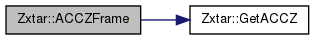
\includegraphics[width=308pt]{class_zxtar_a38c761a822e613fa23fda04c0b947cf0_cgraph}
\end{center}
\end{figure}


\index{\-Zxtar@{\-Zxtar}!\-A\-C\-C\-Z\-Frame\-Average@{\-A\-C\-C\-Z\-Frame\-Average}}
\index{\-A\-C\-C\-Z\-Frame\-Average@{\-A\-C\-C\-Z\-Frame\-Average}!Zxtar@{\-Zxtar}}
\paragraph[{\-A\-C\-C\-Z\-Frame\-Average}]{\setlength{\rightskip}{0pt plus 5cm}double {\bf \-Zxtar\-::\-A\-C\-C\-Z\-Frame\-Average} (
)}\label{class_zxtar_a20d5673fac7f757e102eb2642e4a8066}
\-Method to compute the \-Z-\/axis data frame avarage 

\-Definition at line 403 of file \-Zxtar.\-cpp.

\index{\-Zxtar@{\-Zxtar}!\-A\-C\-C\-Z\-Frame\-Print@{\-A\-C\-C\-Z\-Frame\-Print}}
\index{\-A\-C\-C\-Z\-Frame\-Print@{\-A\-C\-C\-Z\-Frame\-Print}!Zxtar@{\-Zxtar}}
\paragraph[{\-A\-C\-C\-Z\-Frame\-Print}]{\setlength{\rightskip}{0pt plus 5cm}void {\bf \-Zxtar\-::\-A\-C\-C\-Z\-Frame\-Print} (
)}\label{class_zxtar_a868b738a65e5b5cfd4fabe7677208a6e}
\-Method for printing the \-Z-\/axis data frame 

\-Definition at line 390 of file \-Zxtar.\-cpp.

\index{\-Zxtar@{\-Zxtar}!\-A\-C\-C\-Z\-Frame\-Std\-Deviation@{\-A\-C\-C\-Z\-Frame\-Std\-Deviation}}
\index{\-A\-C\-C\-Z\-Frame\-Std\-Deviation@{\-A\-C\-C\-Z\-Frame\-Std\-Deviation}!Zxtar@{\-Zxtar}}
\paragraph[{\-A\-C\-C\-Z\-Frame\-Std\-Deviation}]{\setlength{\rightskip}{0pt plus 5cm}double {\bf \-Zxtar\-::\-A\-C\-C\-Z\-Frame\-Std\-Deviation} (
)}\label{class_zxtar_a05a3069faae3a30873305079dd1fec4a}
\-Method to compute the \-Z-\/axis data frame standard deviation 

\-Definition at line 425 of file \-Zxtar.\-cpp.

\index{\-Zxtar@{\-Zxtar}!\-Available\-A\-C\-C@{\-Available\-A\-C\-C}}
\index{\-Available\-A\-C\-C@{\-Available\-A\-C\-C}!Zxtar@{\-Zxtar}}
\paragraph[{\-Available\-A\-C\-C}]{\setlength{\rightskip}{0pt plus 5cm}void {\bf \-Zxtar\-::\-Available\-A\-C\-C} (
)}\label{class_zxtar_a2700322341a53e4db4250c819218161d}
\-To wait until the data is available by using a while loop 

\-Definition at line 51 of file \-Zxtar.\-cpp.



\-Here is the call graph for this function\-:\nopagebreak
\begin{figure}[H]
\begin{center}
\leavevmode
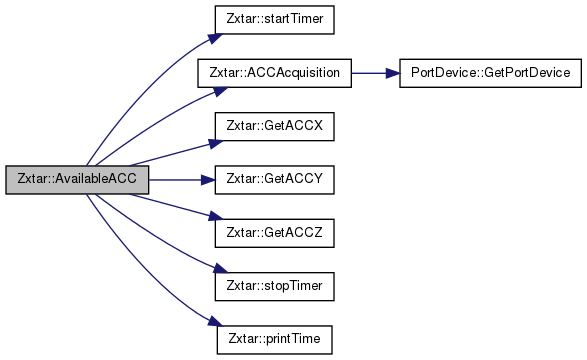
\includegraphics[width=350pt]{class_zxtar_a2700322341a53e4db4250c819218161d_cgraph}
\end{center}
\end{figure}


\index{\-Zxtar@{\-Zxtar}!\-Data\-Rate@{\-Data\-Rate}}
\index{\-Data\-Rate@{\-Data\-Rate}!Zxtar@{\-Zxtar}}
\paragraph[{\-Data\-Rate}]{\setlength{\rightskip}{0pt plus 5cm}void {\bf \-Zxtar\-::\-Data\-Rate} (
\begin{itemize}
\item[{int}]{set\-Rate}
\end{itemize}
)}\label{class_zxtar_acc66525a310d1f24e3d985ac85c846f2}
\-Method to set the \-Data \-Rate 

\-Definition at line 124 of file \-Zxtar.\-cpp.



\-Here is the call graph for this function\-:\nopagebreak
\begin{figure}[H]
\begin{center}
\leavevmode
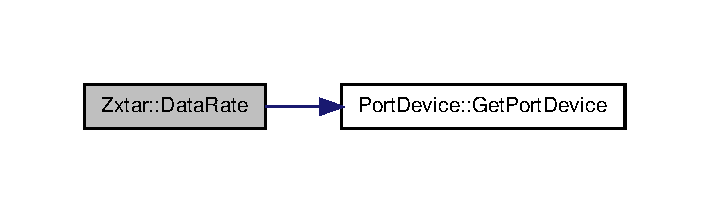
\includegraphics[width=340pt]{class_zxtar_acc66525a310d1f24e3d985ac85c846f2_cgraph}
\end{center}
\end{figure}


\index{\-Zxtar@{\-Zxtar}!\-Get\-A\-C\-C\-X@{\-Get\-A\-C\-C\-X}}
\index{\-Get\-A\-C\-C\-X@{\-Get\-A\-C\-C\-X}!Zxtar@{\-Zxtar}}
\paragraph[{\-Get\-A\-C\-C\-X}]{\setlength{\rightskip}{0pt plus 5cm}double {\bf \-Zxtar\-::\-Get\-A\-C\-C\-X} (
)}\label{class_zxtar_a2d281a6f0b4af1415534315c49310fa2}
\-Method to get \-X-\/axis \-Acceleration 

\-Definition at line 171 of file \-Zxtar.\-cpp.

\index{\-Zxtar@{\-Zxtar}!\-Get\-A\-C\-C\-X\-Frame\-Avarage@{\-Get\-A\-C\-C\-X\-Frame\-Avarage}}
\index{\-Get\-A\-C\-C\-X\-Frame\-Avarage@{\-Get\-A\-C\-C\-X\-Frame\-Avarage}!Zxtar@{\-Zxtar}}
\paragraph[{\-Get\-A\-C\-C\-X\-Frame\-Avarage}]{\setlength{\rightskip}{0pt plus 5cm}double {\bf \-Zxtar\-::\-Get\-A\-C\-C\-X\-Frame\-Avarage} (
)}\label{class_zxtar_a05401473e403950d0ae3f3bd111b0a5e}
\-Method to get the \-X-\/axis data frame avarage 

\-Definition at line 276 of file \-Zxtar.\-cpp.

\index{\-Zxtar@{\-Zxtar}!\-Get\-A\-C\-C\-X\-Frame\-Std\-Deviation@{\-Get\-A\-C\-C\-X\-Frame\-Std\-Deviation}}
\index{\-Get\-A\-C\-C\-X\-Frame\-Std\-Deviation@{\-Get\-A\-C\-C\-X\-Frame\-Std\-Deviation}!Zxtar@{\-Zxtar}}
\paragraph[{\-Get\-A\-C\-C\-X\-Frame\-Std\-Deviation}]{\setlength{\rightskip}{0pt plus 5cm}double {\bf \-Zxtar\-::\-Get\-A\-C\-C\-X\-Frame\-Std\-Deviation} (
)}\label{class_zxtar_a1df7370b9b0a58d1554248b56fdc90e6}
\-Method to get the \-X-\/axis data frame standard deviation 

\-Definition at line 298 of file \-Zxtar.\-cpp.

\index{\-Zxtar@{\-Zxtar}!\-Get\-A\-C\-C\-Y@{\-Get\-A\-C\-C\-Y}}
\index{\-Get\-A\-C\-C\-Y@{\-Get\-A\-C\-C\-Y}!Zxtar@{\-Zxtar}}
\paragraph[{\-Get\-A\-C\-C\-Y}]{\setlength{\rightskip}{0pt plus 5cm}double {\bf \-Zxtar\-::\-Get\-A\-C\-C\-Y} (
)}\label{class_zxtar_ae4a5f6a374a0bf48e62a8066509ddd95}
\-Method to get \-Y-\/axis \-Acceleration 

\-Definition at line 176 of file \-Zxtar.\-cpp.

\index{\-Zxtar@{\-Zxtar}!\-Get\-A\-C\-C\-Y\-Frame\-Avarage@{\-Get\-A\-C\-C\-Y\-Frame\-Avarage}}
\index{\-Get\-A\-C\-C\-Y\-Frame\-Avarage@{\-Get\-A\-C\-C\-Y\-Frame\-Avarage}!Zxtar@{\-Zxtar}}
\paragraph[{\-Get\-A\-C\-C\-Y\-Frame\-Avarage}]{\setlength{\rightskip}{0pt plus 5cm}double {\bf \-Zxtar\-::\-Get\-A\-C\-C\-Y\-Frame\-Avarage} (
)}\label{class_zxtar_a36337fe44ca204e5118ccb09247d2cf4}
\-Method to get the \-Y-\/axis data frame avarage 

\-Definition at line 346 of file \-Zxtar.\-cpp.

\index{\-Zxtar@{\-Zxtar}!\-Get\-A\-C\-C\-Y\-Frame\-Std\-Deviation@{\-Get\-A\-C\-C\-Y\-Frame\-Std\-Deviation}}
\index{\-Get\-A\-C\-C\-Y\-Frame\-Std\-Deviation@{\-Get\-A\-C\-C\-Y\-Frame\-Std\-Deviation}!Zxtar@{\-Zxtar}}
\paragraph[{\-Get\-A\-C\-C\-Y\-Frame\-Std\-Deviation}]{\setlength{\rightskip}{0pt plus 5cm}double {\bf \-Zxtar\-::\-Get\-A\-C\-C\-Y\-Frame\-Std\-Deviation} (
)}\label{class_zxtar_acdb9ddb50f7f932a5a28d9dac4454d0b}
\-Method to get the \-Y-\/axis data frame standard deviation 

\-Definition at line 367 of file \-Zxtar.\-cpp.

\index{\-Zxtar@{\-Zxtar}!\-Get\-A\-C\-C\-Z@{\-Get\-A\-C\-C\-Z}}
\index{\-Get\-A\-C\-C\-Z@{\-Get\-A\-C\-C\-Z}!Zxtar@{\-Zxtar}}
\paragraph[{\-Get\-A\-C\-C\-Z}]{\setlength{\rightskip}{0pt plus 5cm}double {\bf \-Zxtar\-::\-Get\-A\-C\-C\-Z} (
)}\label{class_zxtar_a457606063c02dac5bd51c570f52d17e9}
\-Method to get \-Z-\/axis \-Acceleration 

\-Definition at line 181 of file \-Zxtar.\-cpp.

\index{\-Zxtar@{\-Zxtar}!\-Get\-A\-C\-C\-Z\-Frame\-Avarage@{\-Get\-A\-C\-C\-Z\-Frame\-Avarage}}
\index{\-Get\-A\-C\-C\-Z\-Frame\-Avarage@{\-Get\-A\-C\-C\-Z\-Frame\-Avarage}!Zxtar@{\-Zxtar}}
\paragraph[{\-Get\-A\-C\-C\-Z\-Frame\-Avarage}]{\setlength{\rightskip}{0pt plus 5cm}double {\bf \-Zxtar\-::\-Get\-A\-C\-C\-Z\-Frame\-Avarage} (
)}\label{class_zxtar_ac98474432e60260d18c7d82b98066f38}
\-Method to get the \-Z-\/axis data frame avarage 

\-Definition at line 418 of file \-Zxtar.\-cpp.

\index{\-Zxtar@{\-Zxtar}!\-Get\-A\-C\-C\-Z\-Frame\-Std\-Deviation@{\-Get\-A\-C\-C\-Z\-Frame\-Std\-Deviation}}
\index{\-Get\-A\-C\-C\-Z\-Frame\-Std\-Deviation@{\-Get\-A\-C\-C\-Z\-Frame\-Std\-Deviation}!Zxtar@{\-Zxtar}}
\paragraph[{\-Get\-A\-C\-C\-Z\-Frame\-Std\-Deviation}]{\setlength{\rightskip}{0pt plus 5cm}double {\bf \-Zxtar\-::\-Get\-A\-C\-C\-Z\-Frame\-Std\-Deviation} (
)}\label{class_zxtar_a6c4ec5504080ebbab177a1f135ab9dae}
\-Method to get the \-Z-\/axis data frame standard deviation 

\-Definition at line 445 of file \-Zxtar.\-cpp.

\index{\-Zxtar@{\-Zxtar}!\-Kbhit@{\-Kbhit}}
\index{\-Kbhit@{\-Kbhit}!Zxtar@{\-Zxtar}}
\paragraph[{\-Kbhit}]{\setlength{\rightskip}{0pt plus 5cm}int {\bf \-Zxtar\-::\-Kbhit} (
\begin{itemize}
\item[{void}]{}
\end{itemize}
)}\label{class_zxtar_a49c19995c024562162676a047523b47a}
\-Method for the keyboard hit 

\-Definition at line 70 of file \-Zxtar.\-cpp.

\index{\-Zxtar@{\-Zxtar}!print\-Time@{print\-Time}}
\index{print\-Time@{print\-Time}!Zxtar@{\-Zxtar}}
\paragraph[{print\-Time}]{\setlength{\rightskip}{0pt plus 5cm}void {\bf \-Zxtar\-::print\-Time} (
\begin{itemize}
\item[{double}]{duration}
\end{itemize}
)\hspace{0.3cm}{\ttfamily  [static]}}\label{class_zxtar_a54cab536bc19272a7af54346f0746251}
\-Method to print the timer 

\-Definition at line 218 of file \-Zxtar.\-cpp.

\index{\-Zxtar@{\-Zxtar}!\-Set\-Frame\-Word@{\-Set\-Frame\-Word}}
\index{\-Set\-Frame\-Word@{\-Set\-Frame\-Word}!Zxtar@{\-Zxtar}}
\paragraph[{\-Set\-Frame\-Word}]{\setlength{\rightskip}{0pt plus 5cm}void {\bf \-Zxtar\-::\-Set\-Frame\-Word} (
\begin{itemize}
\item[{unsigned int}]{framevalue}
\end{itemize}
)}\label{class_zxtar_ab1fcbd04a4b7c72c464a18d65bc66826}
\-Method to set the frame word of the acceleration readings 

\-Definition at line 226 of file \-Zxtar.\-cpp.

\index{\-Zxtar@{\-Zxtar}!\-Set\-Sensitivity@{\-Set\-Sensitivity}}
\index{\-Set\-Sensitivity@{\-Set\-Sensitivity}!Zxtar@{\-Zxtar}}
\paragraph[{\-Set\-Sensitivity}]{\setlength{\rightskip}{0pt plus 5cm}void {\bf \-Zxtar\-::\-Set\-Sensitivity} (
\begin{itemize}
\item[{int}]{g\-Sensitivity}
\end{itemize}
)}\label{class_zxtar_a7b07dfc237f67c1e444a8114a1e087ee}
\-Method to select the g-\/range for the accelerometer \-Sensor \-Board \-B\-Y \-S\-E\-N\-D\-I\-N\-G \-A g0 g1 or g2 you are able to change the \-S\-E\-N\-S\-I\-T\-I\-V\-I\-T\-Y g0 = 8g ; g1 = 2g ; g2 = 4g 

\-Definition at line 96 of file \-Zxtar.\-cpp.



\-Here is the call graph for this function\-:\nopagebreak
\begin{figure}[H]
\begin{center}
\leavevmode
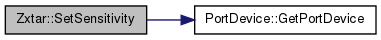
\includegraphics[width=350pt]{class_zxtar_a7b07dfc237f67c1e444a8114a1e087ee_cgraph}
\end{center}
\end{figure}


\index{\-Zxtar@{\-Zxtar}!start\-Timer@{start\-Timer}}
\index{start\-Timer@{start\-Timer}!Zxtar@{\-Zxtar}}
\paragraph[{start\-Timer}]{\setlength{\rightskip}{0pt plus 5cm}void {\bf \-Zxtar\-::start\-Timer} (
)}\label{class_zxtar_a5fdc5fa7aaba3621ba452fd092b79beb}
\-Method to start the timer 

\-Definition at line 197 of file \-Zxtar.\-cpp.

\index{\-Zxtar@{\-Zxtar}!stop\-Timer@{stop\-Timer}}
\index{stop\-Timer@{stop\-Timer}!Zxtar@{\-Zxtar}}
\paragraph[{stop\-Timer}]{\setlength{\rightskip}{0pt plus 5cm}double {\bf \-Zxtar\-::stop\-Timer} (
)}\label{class_zxtar_ac7e152ff3caa185696bdbdab1e245570}
\-Method to stop the timer 

\-Definition at line 202 of file \-Zxtar.\-cpp.



\subsubsection{\-Member \-Data \-Documentation}
\index{\-Zxtar@{\-Zxtar}!\-Z\-S\-T\-A\-R@{\-Z\-S\-T\-A\-R}}
\index{\-Z\-S\-T\-A\-R@{\-Z\-S\-T\-A\-R}!Zxtar@{\-Zxtar}}
\paragraph[{\-Z\-S\-T\-A\-R}]{\setlength{\rightskip}{0pt plus 5cm}{\bf \-Port\-Device} {\bf \-Zxtar\-::\-Z\-S\-T\-A\-R}}\label{class_zxtar_a963d107179ac6801f81b80632bf4e189}
\-Data \-Member for the use fo the \-Port\-Device class with the sensor board 

\-Definition at line 88 of file \-Zxtar.\-h.

    
    
    
  
  
    \section{main.cpp \-File \-Reference}    
{\ttfamily \#include \char`\"{}\-Hridd.\-h\char`\"{}}\*
\-Include dependency graph for main.\-cpp\-:\nopagebreak
\begin{figure}[H]
\begin{center}
\leavevmode
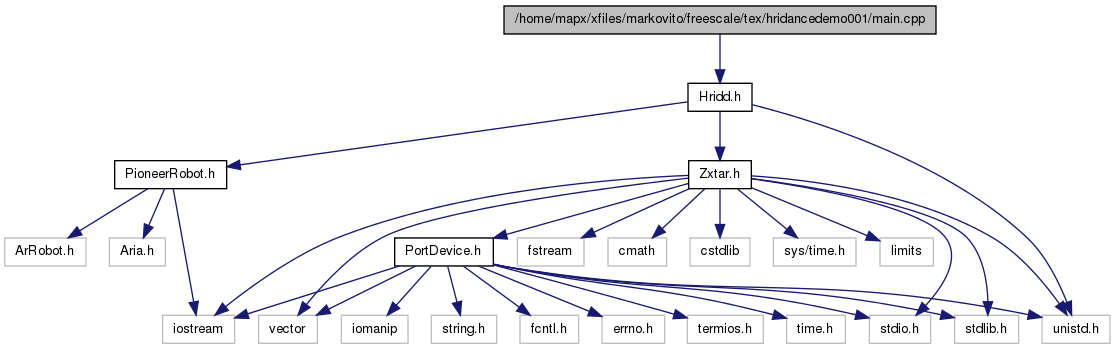
\includegraphics[width=350pt]{main_8cpp__incl}
\end{center}
\end{figure}
\subsubsection*{\-Functions}
\begin{itemize}
\item 
int {\bf main} ()
\end{itemize}

  
  
\subsubsection{\-Function \-Documentation}
\index{main.\-cpp@{main.\-cpp}!main@{main}}
\index{main@{main}!main.cpp@{main.\-cpp}}
\paragraph[{main}]{\setlength{\rightskip}{0pt plus 5cm}int {\bf main} (
)}\label{main_8cpp_ae66f6b31b5ad750f1fe042a706a4e3d4}


\-Definition at line 3 of file main.\-cpp.



\-Here is the call graph for this function\-:\nopagebreak
\begin{figure}[H]
\begin{center}
\leavevmode
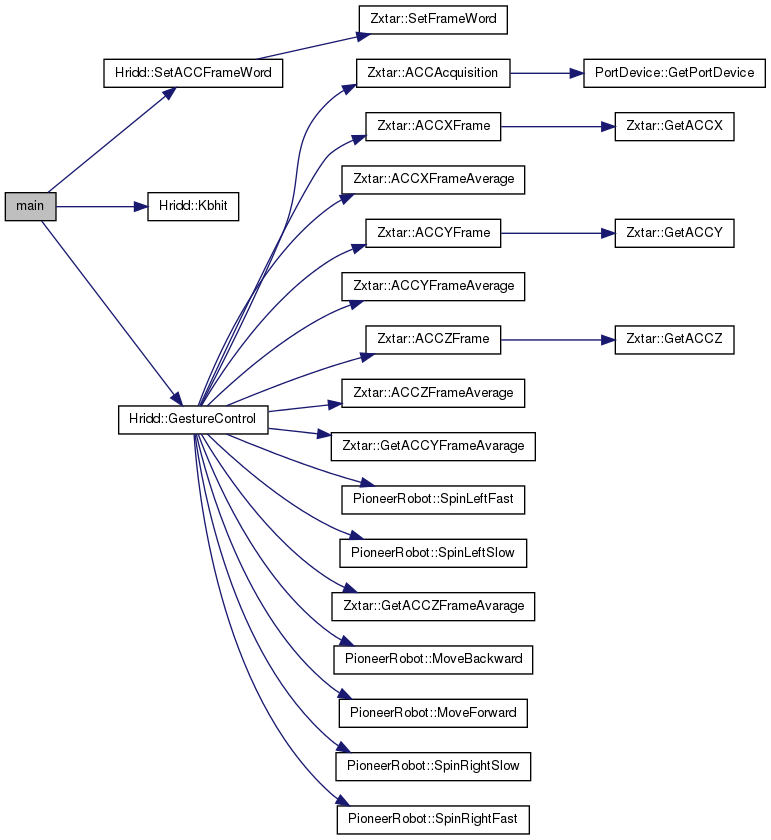
\includegraphics[width=350pt]{main_8cpp_ae66f6b31b5ad750f1fe042a706a4e3d4_cgraph}
\end{center}
\end{figure}



  
  
  
  
\end{appendices}

